\documentclass[a4paper]{article}
\linespread{1.6}
\usepackage{enumerate}
\usepackage{geometry}
\usepackage{setspace}
\usepackage{amsmath}
\usepackage{amssymb}
\usepackage[pdftex]{graphicx}
\usepackage{float}
\usepackage{subfigure}
\usepackage{listings}
\geometry{left=1.4cm,right=1.4cm,top=2.5cm,bottom=2.5cm}

\begin{document}
\begin{spacing}{2.0}
\begin{flushleft}\begin{huge}EEL5840 Fundamental Machine Learning   Homework 3\end{huge}\end{flushleft}
\begin{flushright}\begin{Large} Hudanyun Sheng \end{Large}\end{flushright}

\Large{All the code used are attached at the end of this report.}

\paragraph{\huge\textbf{ Question 1\\} }
\normalsize
\textbf{1.1}  
	 Based on my result, the combination of parameters \textbf{filter} and \textbf{regularization parameter} which gives the best mean square error in the 	validation is $\lambda = 0.1$, filter order $D = 4$.\\
	 The plots of the performance of validation set regarding to filter order and regularization parameter are shown below: 
	 \begin{figure}[H]
	    \centering
	        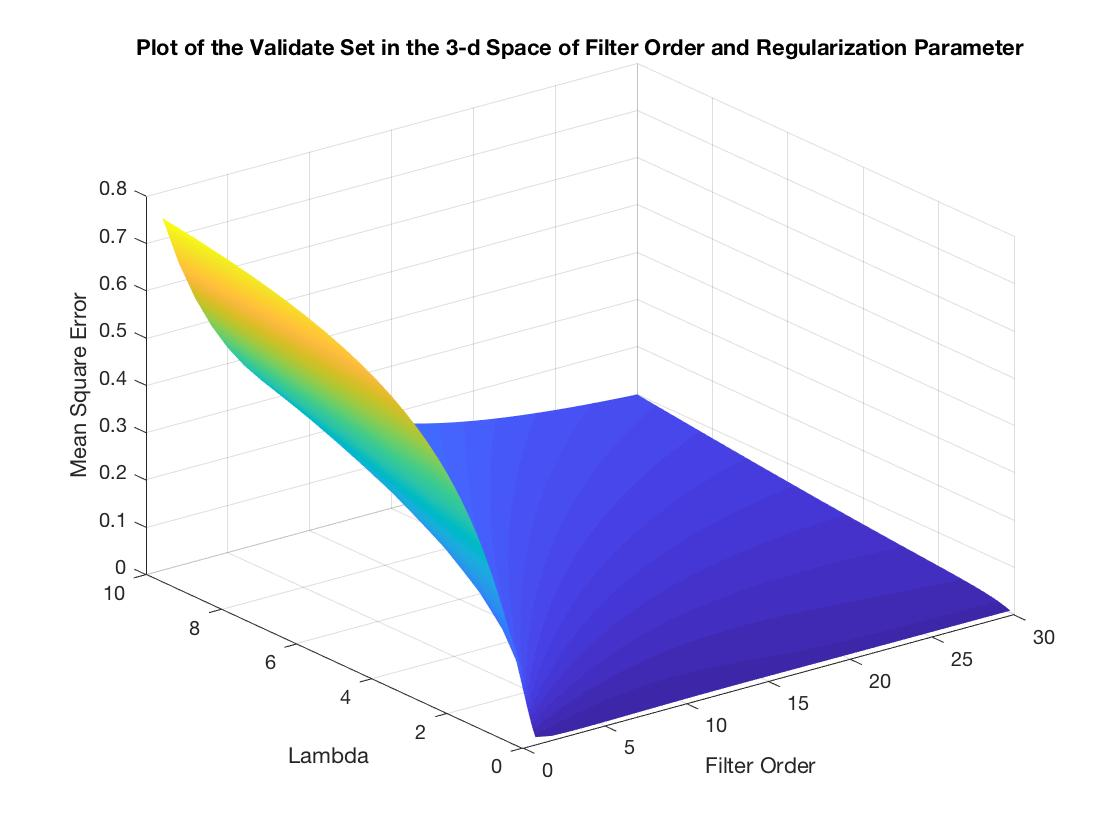
\includegraphics[width=6in]{1_1_2.jpg}
	        \caption{3-d plot of the performance of validate set in the space of filter order and regularization parameter}
	        \label{fig:side:a}
	  \end{figure}
	As my experiment goes, I change the filter order from 1 to 30, and $\lambda$ one of the 50 numbers obtained in $[0.1, 10]$, and I got the minimum MSE is obtained when $\lambda = 0.1$ and $M = 4$. While if I change the range of $\lambda$ to be $[10^{-5}, 10^{-3}]$, the minimum MSE is obtained when $\lambda = 10^{-5}$ and $M = 20$. So the best regularization term and best filter order depend on each other.\\
	When filter order is small, we do not need large regularization term, that is the reason the error gets a big value when we have a small filter order with 	a large value of regularization term.\\
	
\textbf{1.2} 
	With regularization parameter $\lambda = 0.1$, using filter orders 4, 8, 30. The MSE of the test noisy data, are respectively 1.3521, 1.2249, 1.2166, respectively. The filtering results are shown below:
	\begin{figure}[H]
	    \centering
	        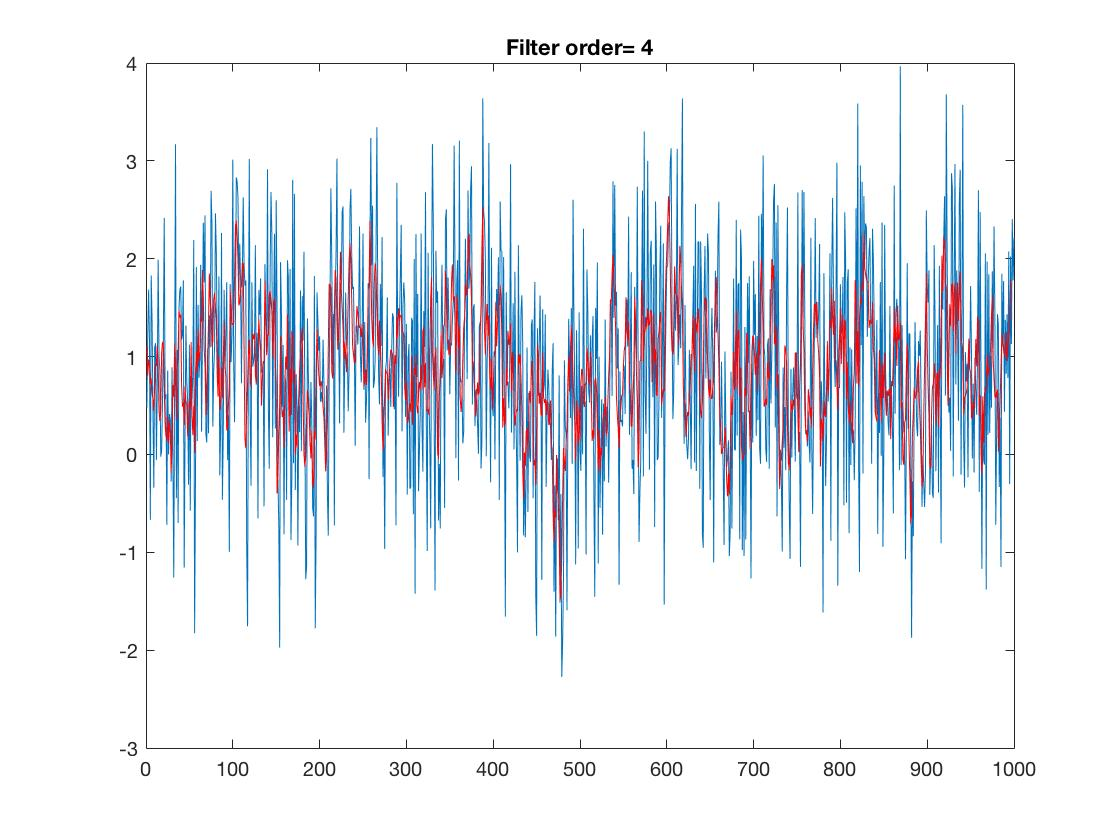
\includegraphics[width=4.5in]{1_2_2.jpg}
	        \caption{Filtering result using filter order 4}
	        \label{fig:side:a}
	  \end{figure}
	  
	  \begin{figure}[H]
	    \centering
	        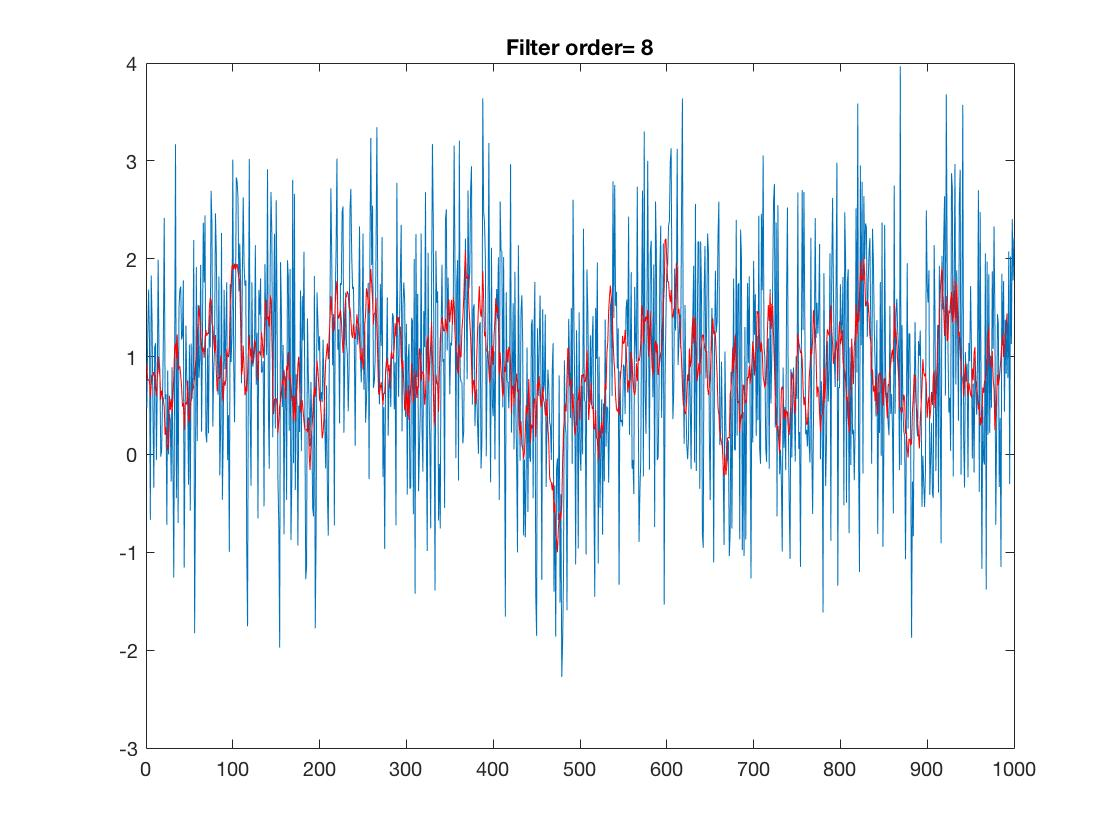
\includegraphics[width=4.5in]{1_2_3.jpg}
	        \caption{Filtering result using filter order 8}
	        \label{fig:side:a}
	  \end{figure}
	  
	\begin{figure}[H]
	    \centering
	        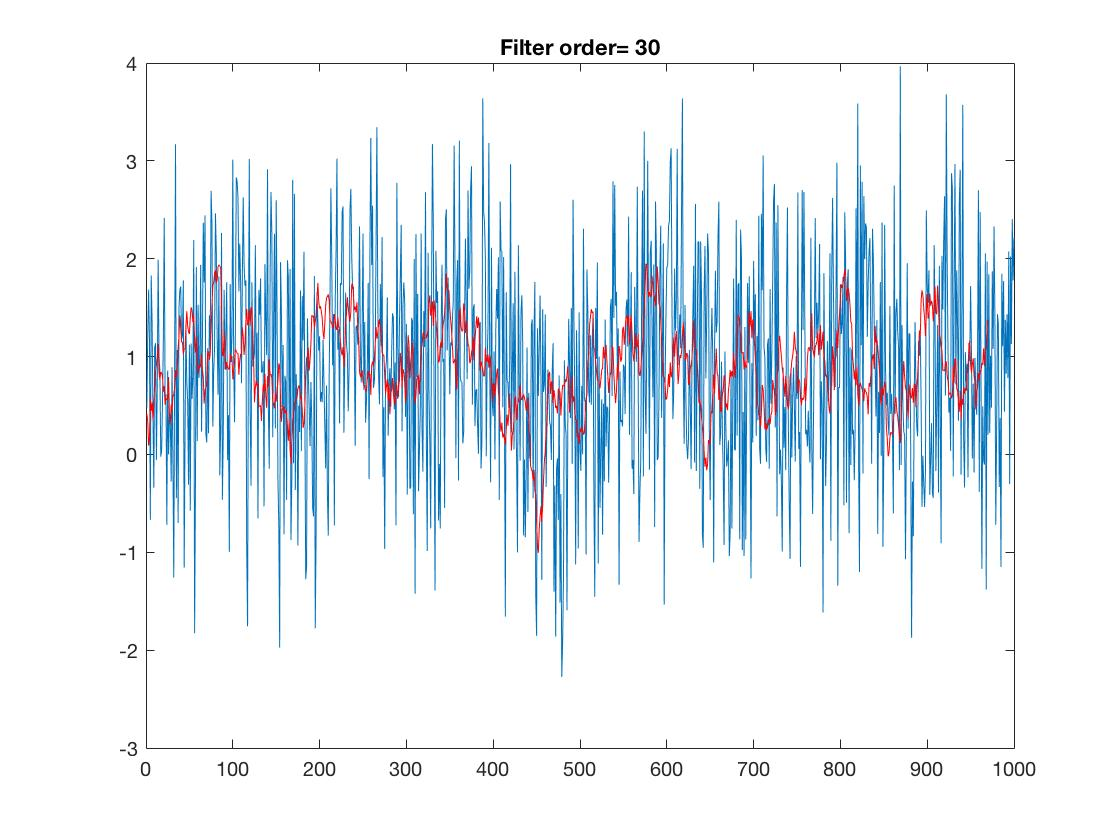
\includegraphics[width=4.5in]{1_2_4.jpg}
	        \caption{Filtering result using filter order 30}
	        \label{fig:side:a}
	\end{figure}
	Based on the result, order filter 30 has the best performance, it works better for this noisy data, and gets the smallest MES at the same time.
\paragraph{\huge\textbf{ Question 2\\} }

\normalsize
\noindent

\textbf{2.1} 

I changed $\eta$ between $10^{-7}$ and $10^{-6}$, and changing filter orders between 1 and 30. Based on my result, the best performance regarding validate set happens when filter order $M = 12$, $\eta = 10^{-6}$. If I instead change $\eta$ between $10^{-7}$ and $10^{-5}$, the best performance regarding validate set happens when filter order $M = 2$, $\eta = 10^{-5}$. And I later used $\eta = 10^{-6}$ to quantify the performance in the MSE-sense using filter orders 4, 8, and 30 in the noisy data. \\
With step size $\eta = 10^{-6}$, filter order $M = 4, 8, 30$ respectively, the MSE calculated for the validation set are 0.1133 (for $M = 4$), 0.0187 (for $M = 8$), 0.0280 (for $M = 30$), which we can see, based on the validate set, the filter order $M =8$ gets the minimum value of MSE. The figures of the test signal are shown below:

\begin{figure}[H]
	\centering
	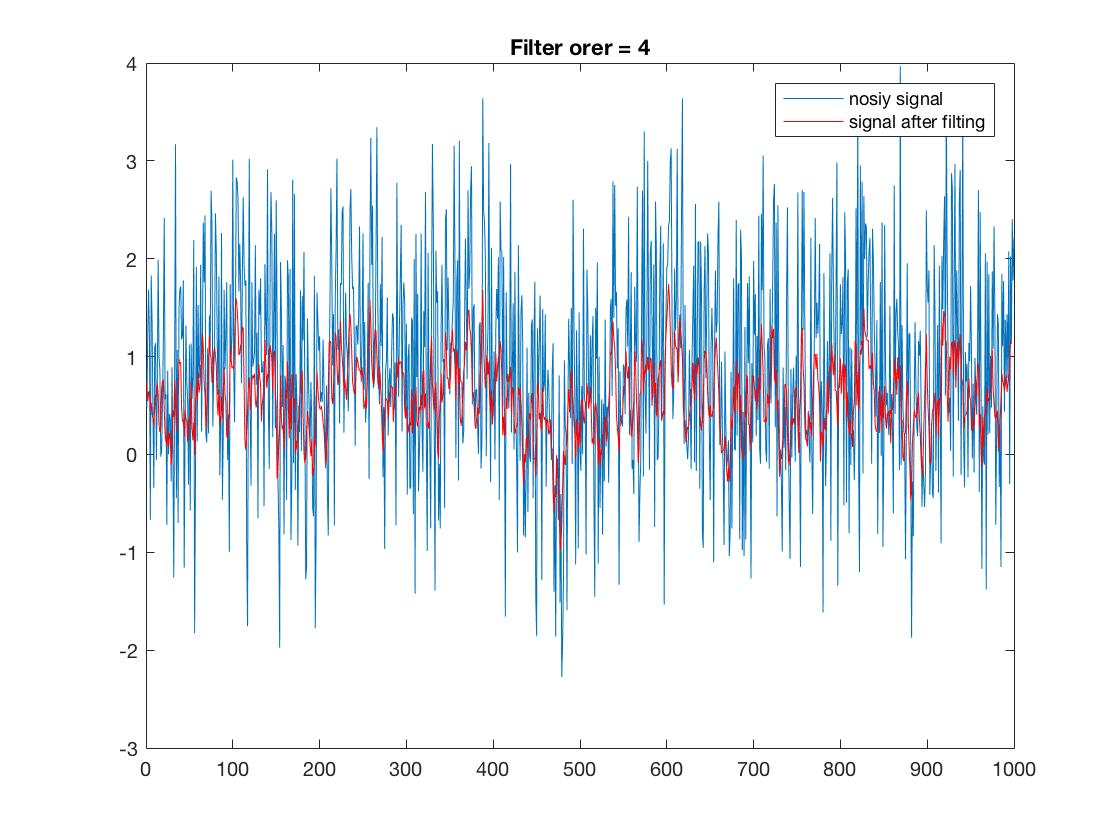
\includegraphics[width=5in]{2_1_4.jpg}
	\caption{Filtering result using filter order 4}
	\label{fig:side:a}
	\end{figure}
	  
\begin{figure}[H]
	\centering
	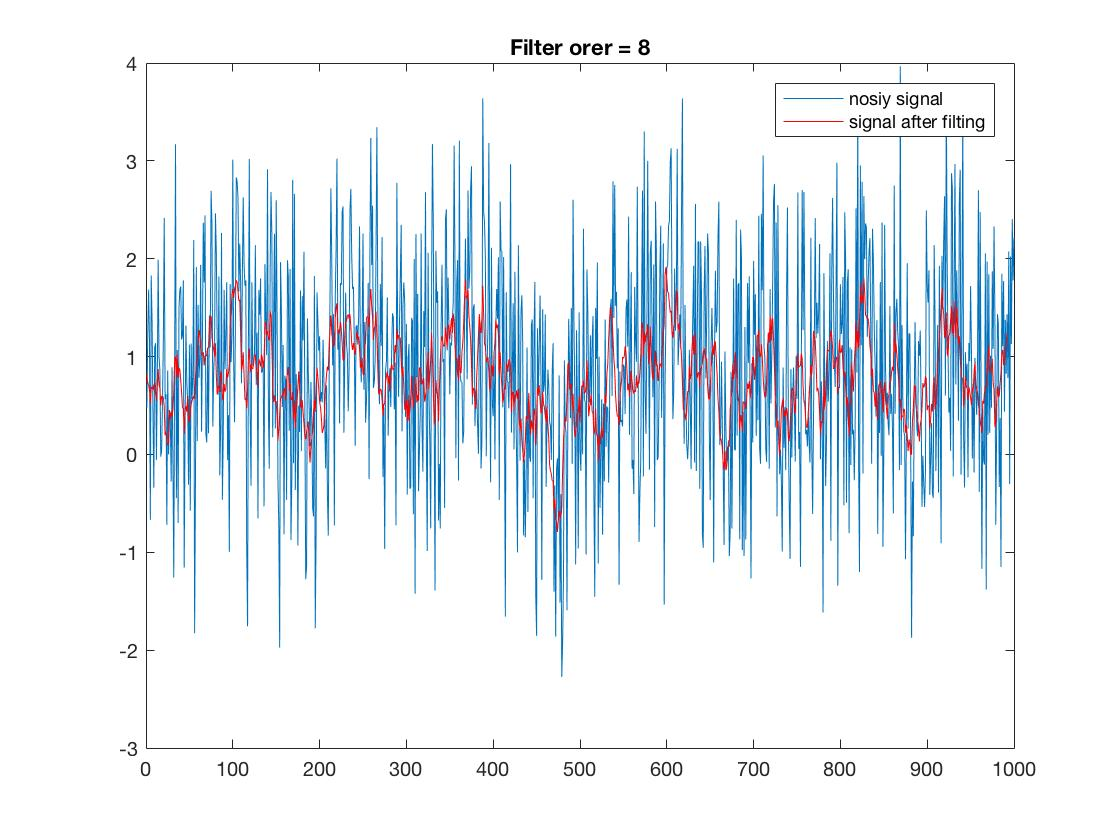
\includegraphics[width=5in]{2_1_8.jpg}
	\caption{Filtering result using filter order 8}
	\label{fig:side:a}
\end{figure}

\begin{figure}[H]
	\centering
	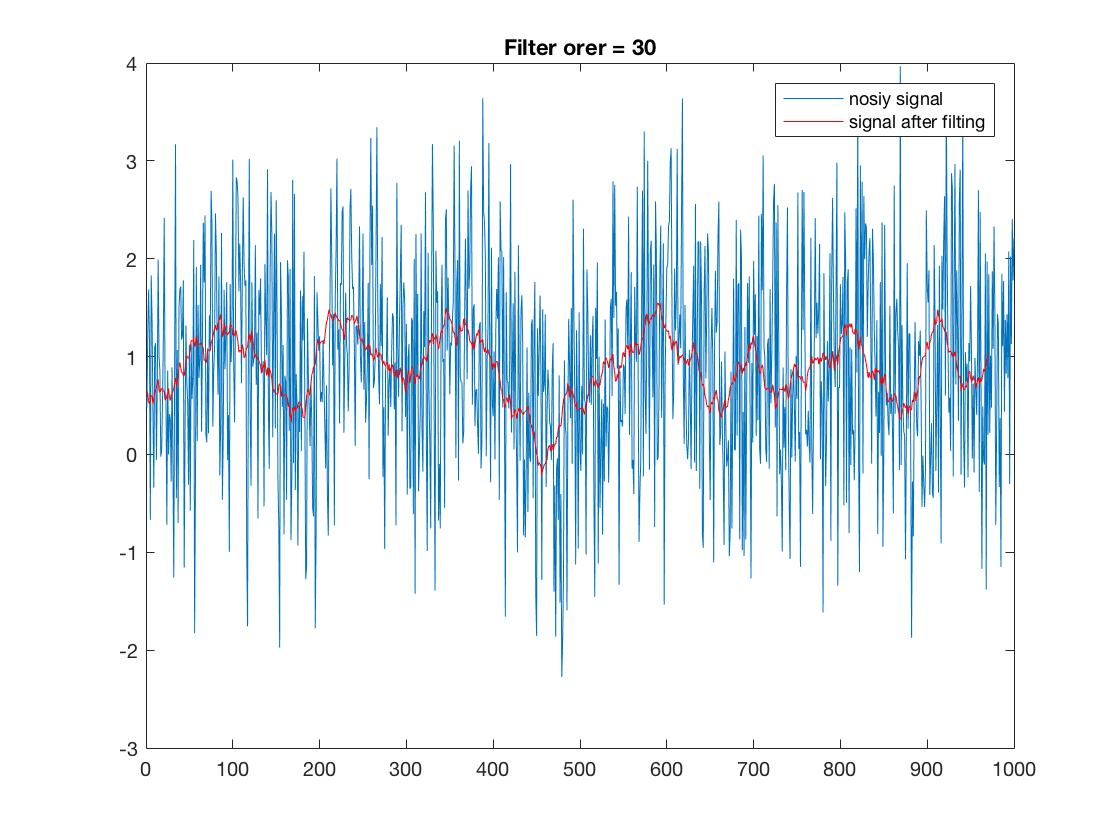
\includegraphics[width=5in]{2_1_30.jpg}
	\caption{Filtering result using filter order 30}
	\label{fig:side:a}
\end{figure}

With the figures shown, we can see that visually, the filter order $M=30$ works the best, since it removes most of the noise. Regarding the MSE calculated for the test set, they are 1.3202 (for $M = 4$), 1.2095 (for $M = 8$), and 1.1736 (for $M = 30$). We may conclude that the performance of a filter can not be measured only based on the MSE of the result.\\

\textbf{2.2}  
	I chose the fixed filter model order $M = 4$, change the step size in $\{10^{-9}, 10^{-7}, 10^{-5}, 10^{-3}\}$. The results are shown in figures regarding learning curves and weight tracks:\\
	\begin{figure}[H]
	    \begin{minipage}[t]{0.5\textwidth}
	        \centering
	        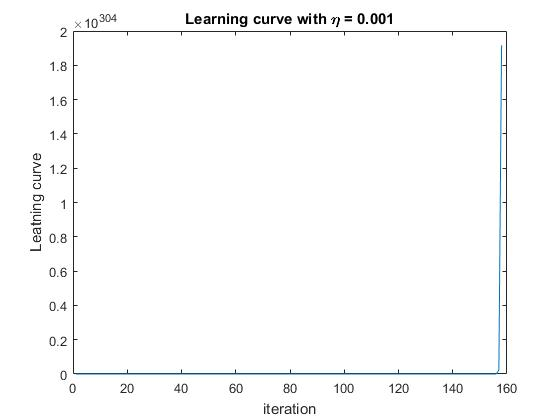
\includegraphics[width=3.4in]{LC_3.jpg}
	        \caption{Learning curve with $\eta = 0.001$}
	        \label{fig:side:a}
	    \end{minipage}%
	  \begin{minipage}[t]{0.5\textwidth}
	      \centering
	      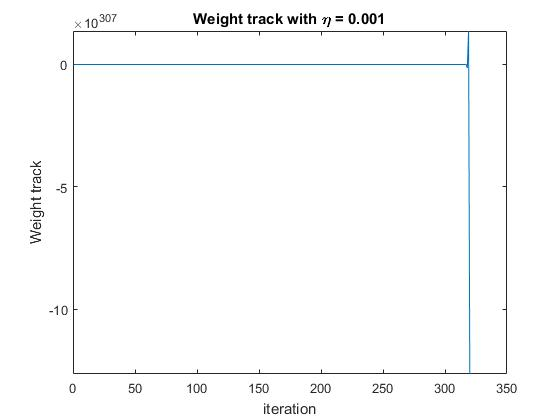
\includegraphics[width=3.4in]{WT_3.jpg}
	      \caption{Weight track with $\eta = 0.001$}
	      \label{fig:side:b}
	    \end{minipage}
	\end{figure}
	
	\begin{figure}[H]
	    \begin{minipage}[t]{0.5\textwidth}
	        \centering
	        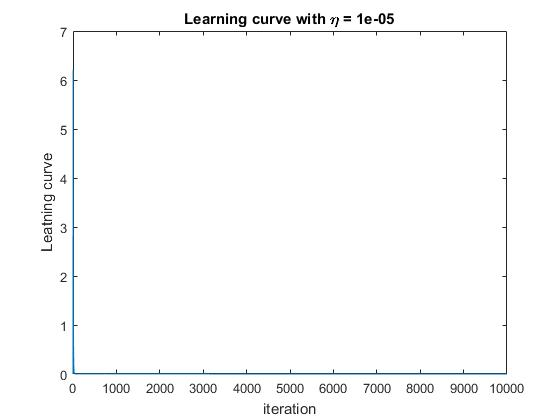
\includegraphics[width=3.4in]{LC_5.jpg}
	        \caption{Learning curve with $\eta = 10^{-5}$}
	        \label{fig:side:a}
	    \end{minipage}%
	  \begin{minipage}[t]{0.5\textwidth}
	      \centering
	      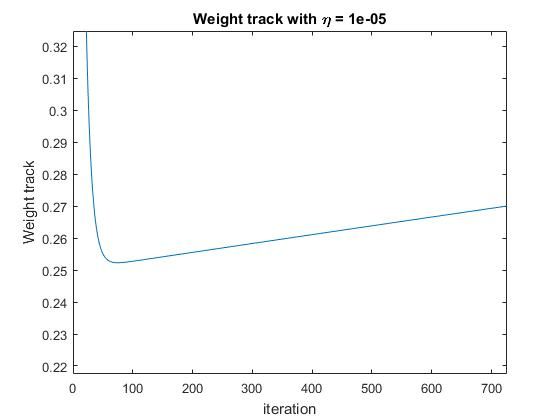
\includegraphics[width=3.4in]{WT_5.jpg}
	      \caption{Weight track with $\eta = 10^{-5}$}
	      \label{fig:side:b}
	    \end{minipage}
	\end{figure}
	
	\begin{figure}[H]
	    \begin{minipage}[t]{0.5\textwidth}
	        \centering
	        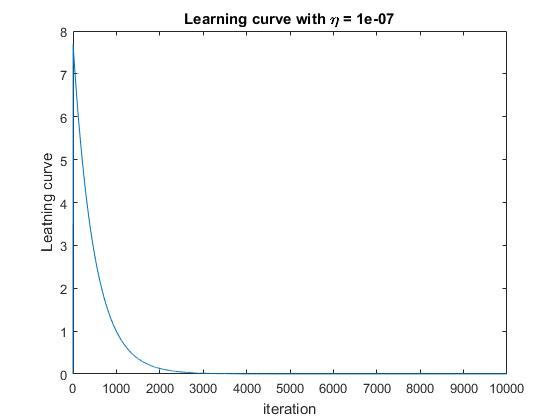
\includegraphics[width=3.4in]{LC_7.jpg}
	        \caption{Learning curve with $\eta = 10^{-7}$}
	        \label{fig:side:a}
	    \end{minipage}%
	  \begin{minipage}[t]{0.5\textwidth}
	      \centering
	      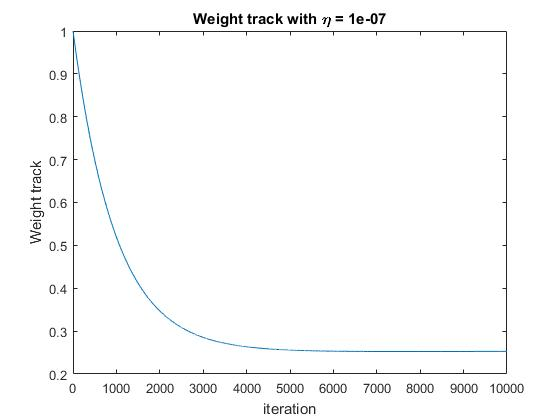
\includegraphics[width=3.4in]{WT_7.jpg}
	      \caption{Weight track with $\eta = 10^{-7}$}
	      \label{fig:side:b}
	    \end{minipage}
	\end{figure}
	
	\begin{figure}[H]
	    \begin{minipage}[t]{0.5\textwidth}
	        \centering
	        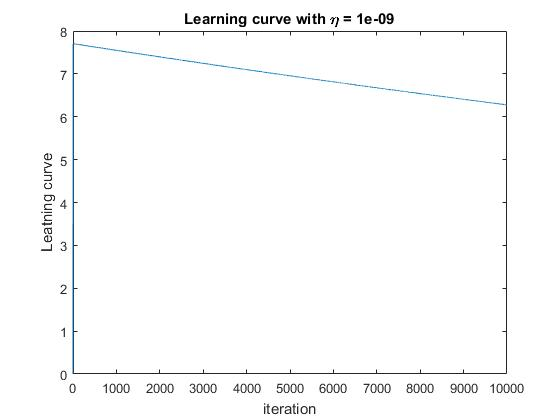
\includegraphics[width=3.4in]{LC_9.jpg}
	        \caption{Learning curve with $\eta = 10^{-9}$}
	        \label{fig:side:a}
	    \end{minipage}%
	  \begin{minipage}[t]{0.5\textwidth}
	      \centering
	      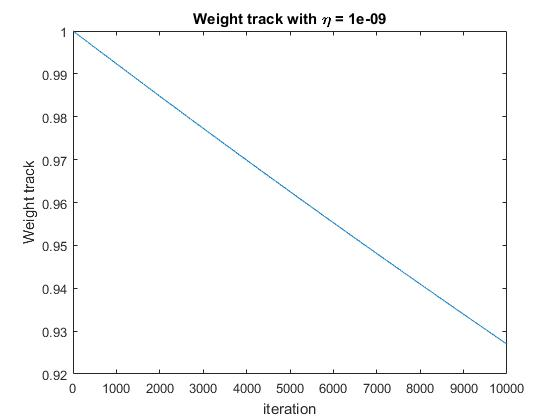
\includegraphics[width=3.4in]{WT_9.jpg}
	      \caption{Weight track with $\eta = 10^{-9}$}
	      \label{fig:side:b}
	    \end{minipage}
	\end{figure}
	Based on the results shown in the figures, we learn that when the step size is too large (i.e.$\eta = 0.001$), the procedure is unable to converge; while if the step size is too small (i.e. $\eta = 10^{-9}$), the procedure seems to approaching convergence, but not within specific iterations. \\
	The compromise between learning time and accuracy should be made. If choosing a large step size, it could end up with no optimal solution found, due to not able to converge; while if choosing a small step size, it will always lead to an optimal solution, but if the step is too small, the calculation time is ignorable. So experience as well as experiment are needed when choosing the step size.


\newpage
\huge{MATLAB code used to complete this report\\}
\normalsize
\textbf{1.1 code}:
\begin{lstlisting}
clear
close all
clc
load('training.txt') % load the training data
load('validate.txt') % load the validate data
load('testnoisy.txt') % load the test data
M_max = 30; % set the max number of filter order
% lambda_list = 10.^(linspace(-5,-1,10)); % set the list of lambda values
lambda_list = logspace(-1,1,50);
J = zeros(size(1:M_max,2), size(lambda_list,2));
for M = 1:M_max
    for lambda_idx = 1:size(lambda_list,2)
        lambda = lambda_list(lambda_idx);
        N_training = size(training,1);
        X_training = zeros(N_training-M, M);
        d_training = zeros(N_training-M, 1);
        for i = 1:(N_training-M)
            X_training(i,:) = training(M-1+i:-1:i);
            d_training(i,:) = training(M+i);
        end
        R = X_training'*X_training/(N_training-M);
        P = X_training'*d_training/(N_training-M);
        w = inv(R+lambda*eye(M))*P;       
        N_validate = size(validate,1);
        X_validate = zeros(N_validate-M, M);
        d_validate = zeros(N_validate-M, 1);
        for i = 1:N_validate-M
            X_validate(i,:) = validate(M-1+i:-1:i);
            d_validate(i,:) = validate(M+i);
        end
        J(M,lambda_idx) = sum((d_validate - X_validate * w).^2)/(N_validate-M);
        ww{M}(:,lambda_idx) = w;
    end
end
min_J = min(min(J));
[best_M_idx, best_lambda_idx] = find(J == min_J);
best_lambda = lambda_list(best_lambda_idx); % lambda which gives the minimum MSE of validate set
best_M = best_M_idx; % filter order which gives the minimum MSE of the validate set
best_w = ww{best_M}(:,best_lambda_idx); % weght which gives the minimum MSE of the validate set
figure
[X,Y] = meshgrid(lambda_list,1:M_max); 
surf(Y, X, J)
shading interp
xlabel('Filter Order')
ylabel('Lambda')
zlabel('Mean Square Error')
title('Plot of the Validate Set in the 3-d Space of Filter Order and Regularization Parameter')
N_testnoisy = size(testnoisy,1);
X_testnoisy = zeros(N_testnoisy-best_M, best_M);
d_testnoisy = zeros(N_testnoisy-best_M, 1);
for i = 1:N_testnoisy-best_M
    X_testnoisy(i,:) = testnoisy(best_M-1+i:-1:i);
	d_testnoisy(i,:) = testnoisy(best_M+i);
end
figure
contourf(lambda_list, 1:M_max, J)
shading interp
x3 = 1:1000;
figure
plot(testnoisy)
hold on
plot(X_testnoisy * best_w, 'r')
title('noisy test data')
legend('noisy test data', 'the result after filtering')
\end{lstlisting}

\newpage
\textbf{1.2 code}:
\begin{lstlisting}
clear
close all
clc
load('training.txt') % load the training data
load('validate.txt') % load the validate data
load('testnoisy.txt') % load the test data
M_list = [4 8 30];
J = zeros(size(M_list,2),1);
% lambda_list = logspace(-10,1,50);
lambda_list = 0.1;
for lambda_idx = 1:size(lambda_list,2)
    lambda = lambda_list(lambda_idx);
    for i = 1:size(M_list,2)
        M = M_list(i);
        N_training = size(training,1);
        X_training = zeros(N_training-M, M);
        d_training = zeros(N_training-M, 1);
        for j = 1:(N_training-M)
            X_training(j,:) = training(M-1+j:-1:j);
            d_training(j,:) = training(M+j);
        end
        R = X_training'*X_training/(N_training-M);
        P = X_training'*d_training/(N_training-M);
        w = inv(R+lambda*eye(M))*P;
        N_validate = size(validate,1);
        X_validate = zeros(N_validate-M, M);
        d_validate = zeros(N_validate-M, 1);
        for j = 1:N_validate-M
            X_validate(j,:) = validate(M-1+j:-1:j);
            d_validate(j,:) = validate(M+j);
        end
        J(i,lambda_idx) = sum((d_validate - X_validate * w).^2)/N_validate;
        ww{i}(:,lambda_idx) = w;
    end
end
figure
for order = 1:3
    plot(lambda_list, J(order,:))
    hold on
end
legend('filter order = 4', 'filter order = 8', 'filter order = 30')
figure
for order = 1:3
    plot(J(order,:))
    hold on
end
legend('filter order = 4', 'filter order = 8', 'filter order = 30')
Jmin = min(J);
[best_order, ~] = find(J == Jmin);
x3 = 1:1000;
for idx_M = 1:size(M_list,2)
    M = M_list(idx_M);
    N_testnoisy = size(testnoisy,1);
    X_testnoisy = zeros(N_testnoisy-M, M);
    d_testnoisy = zeros(N_testnoisy-M, 1);
    for i = 1:N_testnoisy-M
        X_testnoisy(i,:) = testnoisy(M-1+i:-1:i);
        d_testnoisy(i,:) = testnoisy(M+i);
    end
    X_out = X_testnoisy * ww{idx_M};
	J(idx_M) = sum((d_testnoisy - X_out).^2)/(N_testnoisy-M);
    figure
    plot(testnoisy)
    hold on
    plot(X_out,'r')
    title(['Filter order= ' num2str(M)])
\end{lstlisting}	

\newpage
\textbf{2.1 code}: 
\begin{lstlisting}
clear
close all
clc
load('training.txt')
load('validate.txt')
load('testnoisy.txt')
max_iter = 100;
max_M = 30;
% M_list = [4 8 30];
M_list = 1:max_M;
ita_list = logspace(-7, -5);
% ita_list = 10^(-6);
J_validate = zeros(size(M_list,2), size(ita_list,2));
J_test = zeros(size(M_list,2), size(ita_list,2));
for M_idx = 1:size(M_list,2)
    M = M_list(M_idx);
	N_training = size(training,1);
    X_training = zeros(N_training-M, M);
    d_training = zeros(N_training-M, 1);
    for i = 1:(N_training-M)
        X_training(i,:) = training(M-1+i:-1:i);
        d_training(i,:) = training(M+i);
    end
    w = zeros(M,1);
    epsilon = d_training - X_training * w;
    N_validate = size(validate,1);
    X_validate = zeros(N_validate-M, M);
    d_validate = zeros(N_validate-M, 1);
    for i = 1:(N_validate-M)
        X_validate(i,:) = validate(M-1+i:-1:i);
        d_validate(i,:) = validate(M+i);
    end
    for ita_idx = 1:size(ita_list,2)
        w = zeros(M, 1);
        epsilon = d_training - X_training * w;
        ita = ita_list(ita_idx);
        for iter = 1:max_iter
            w_old = w;
            epsilon_old = epsilon;
            w = w_old + (ita * epsilon_old' *X_training)';
            epsilon = d_training - X_training * w;
        end
        J_validate(M_idx,ita_idx) = sum((d_validate - X_validate * w).^2)/(N_validate-M);
        ww{M_idx}(:,ita_idx) = w;
    end
    N_testnoisy = size(testnoisy,1);
    X_testnoisy = zeros(N_testnoisy-M, M);
    d_testnoisy = zeros(N_testnoisy-M, 1);
    for i = 1:(N_testnoisy-M)
        X_testnoisy(i,:) = testnoisy(M-1+i:-1:i);
        d_testnoisy(i,:) = testnoisy(M+i);
    end
%     J_test(M_idx,ita_idx) = sum((d_testnoisy - X_testnoisy * ww{M_idx}).^2)/(N_testnoisy-M);
    X_out = X_testnoisy*ww{M_idx};
    figure
    plot(testnoisy)
    hold on
    plot(X_out, 'r')
    title(['Filter orer = ' num2str(M_list(M_idx))])
    legend('nosiy signal', 'signal after filting')
end
min_J = min(min(J_validate));
[best_M_idx, best_ita_idx] = find(J_validate == min_J);
best_M = M_list(best_M_idx);
best_ita = ita_list(best_ita_idx);
\end{lstlisting}	

\newpage
\textbf{2.2 code}:
\begin{lstlisting}
clear
close all
clc
load('training.txt')
load('validate.txt')
load('testnoisy.txt')
M = 4;
%% training
N_training = size(training,1);
X_training = zeros(N_training-M, M);
d_training = zeros(N_training-M, 1);
for i = 1:(N_training-M)
    X_training(i,:) = training(M-1+i:-1:i);
    d_training(i,:) = training(M+i);
end
%% validate
N_validate = size(validate,1);
X_validate = zeros(N_validate-M, M);
d_validate = zeros(N_validate-M, 1);
for i = 1:N_validate-M
	X_validate(i,:) = validate(M-1+i:-1:i);
	d_validate(i,:) = validate(M+i);
end
%% testnoisy
N_testnoisy = size(testnoisy,1);
X_testnoisy = zeros(N_testnoisy-M, M);
d_testnoisy = zeros(N_testnoisy-M, 1);
for i = 1:N_validate-M
	X_testnoisy(i,:) = validate(M-1+i:-1:i);
	d_testnoisy(i,:) = validate(M+i);
end
%%
ita_list = 10.^(-3:-1:-9);
max_iter = 10000;
J_validate = zeros(size(ita_list,2), max_iter);
ww = cell(1,4);
epsilon_all = cell(1,4);
for ita_idx = 1:size(ita_list,2)
    ita = ita_list(ita_idx);
    ww{ita_idx}(:,1) = ones(M,1);
    epsilon_all{ita_idx}(:,1) = d_training - X_training*ww{ita_idx}(:,1);
    
    for iter = 1:max_iter-1
%         w_old = w;
%         epsilon_old = epsilon;
        ww{ita_idx}(:,iter+1) = ww{ita_idx}(:,iter) + (ita * epsilon_all{ita_idx}(:,iter)' *X_training)';
        epsilon_all{ita_idx}(:,iter+1) = d_training - X_training *  ww{ita_idx}(:,iter+1);
        J_validate(ita_idx, iter+1) = sum((d_training - X_training * ww{ita_idx}(:,iter+1)).^2)/(N_training - M);
    end
end
%%

for ita_idx = 1:size(ita_list,2)
    figure
    plot(1:max_iter, J_validate(ita_idx,:))
    title(['Learning curve with \eta = ' num2str(ita_list(ita_idx))])
    xlabel('iteration')
    ylabel('Leatning curve')
end

for ita_idx = 1:size(ita_list,2)
    figure
    plot(1:max_iter, ww{ita_idx}(1,:))
    title(['Weight track with \eta = ' num2str(ita_list(ita_idx))])
	xlabel('iteration')
    ylabel('Weight track')
end
\end{lstlisting}

\end{spacing}
\end{document}